\chapter{\huge Metodo Runge-Kutta}

\textit{In analisi numerica i metodi Runge-Kutta sono una famiglia di metodi iterativi impliciti ed espliciti per la risuluzione approssimata di equazioni differenziali ordinarie (ODE). Il più comune di questi metodi è il cosidetto ``RK4'' o anche Runge-Kutta del quarto ordine.}
\\\\
Sia dato il problema di Cauchy
\begin{center}
$ \dot y = f(t, y), \quad y(t_0) = y_0.$
\end{center}
Si assume che il tempo sia discretizzato in istanti $t_n$ equidistanziati di un intervallo $h$.\\
Il metodo RK4 per questo problema è allora dato dalle seguenti equazioni:
\begin{eqnarray*}
y_{n+1} &=& y_n + \tfrac{1}{6} \left(k_1 + 2k_2 + 2k_3 + k_4 \right)\\
t_{n+1} &=& t_n + h
\end{eqnarray*}
dove $y_{n+1}$ è l'approssimazione RK4 di $y(t_{n+1})$, e
\begin{eqnarray*}
k_1 &=& hf(t_n, y_n),\\
k_2 &=& hf(t_n + \tfrac{1}{2}h , y_n + \tfrac{1}{2} k_1),\\
k_3 &=& hf(t_n + \tfrac{1}{2}h , y_n + \tfrac{1}{2} k_2),\\
k_4 &=& hf(t_n + h , y_n + k_3).
\end{eqnarray*}
Il valore della funzione $y$ all'istante $t_{n+1}$ è uguale quindi al suo valore all'istante $t_n$ incrementato della media ponderata di quattro incrementi $k$, dove ogni incremento è il prodotto della dimensione dell'intervallo $h$ ed una stimata pendenza specificata dalla funzione $f$.
\begin{itemize}
\item $k_1$ è l'incremento basato sulla pendenza di $f$ all'estremo sinistro dell'intervallo, calcolato in $y_n$ (metodo di Eulero);
\item $k_2$ è l'incremento basato sulla pendenza nel punto medio dell'intervallo, calcolato in $y_n+\frac{1}{2}k_1$;
\item $k_3$ è ancora l'incremento basato sulla pendenza nel punto medio, calcolato però in $y_n+\frac{1}{2}k_2$;
\item $k_4$ è l'ncremento basato sulla pendenza all'estremo destro dell'intervallo, calcolato in $y_n+k_3$.
\end{itemize}
Si nota dalla formula per $y_{n+1}$ che peso maggiore viene assegnato all'incremento al centro dell'intervallo. Inoltre, se $f=f(t)$ cioè non dipende da $y$, il metodo RK4 si riduce alla regola di integrazione di Simpson.

RK4 è un metodo del quarto ordine e quindi l'errore ad ogni step è dell'ordine di $h^5$, mentre l'errore totale accumulato è dell'ordine di $h^4$.

\section{Il Pendolo Caotico}
Il sistema che si intende simulare è quello dell'oscillatore caotico forzato di equazione
\begin{center}
$\ddot{\theta} = \underbrace{\frac{g}{R}}_1 \sin(\theta)-\underbrace{\frac{k}{m}}_q \dot{\theta}+\underbrace{\frac{f}{mR}}_b \cos(\omega t)$.
\end{center}
È possibile rielaborare l'equazione precedente in un sistema di equazioni differenziali del primo ordine come di seguito
$$\begin{system}
\dot\theta&=\phi \\[1ex] \dot\phi&=\sin(\theta)-q\phi+b\cos(\omega t)
\end{system}$$
ed applicare ora la formula del metodo RK4 ad entrambe le equazioni.
\\

Rappresentando la traiettoria del sistema nello spazio delle fasi si ottiene
\begin{figure}[H]
\centering
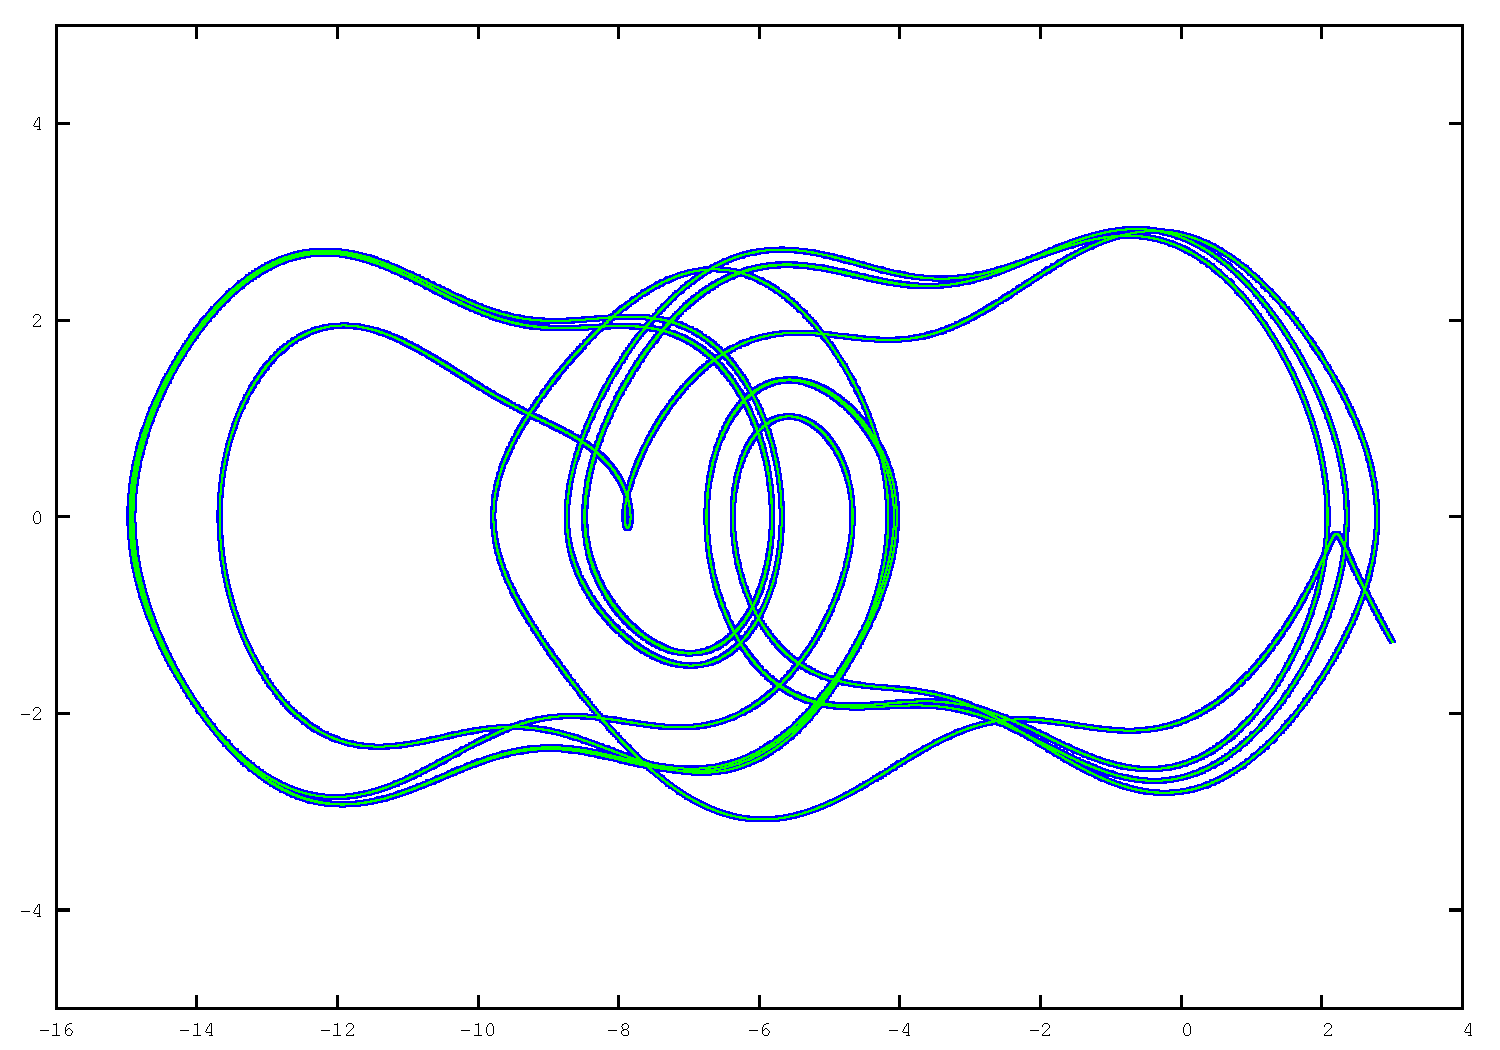
\includegraphics[width=0.75\textwidth]{chaotic}
\caption{Traiettoria dell'oscillatore per $q = 0.3$, $b = 1.4$, $\omega = 0.6667$}
\label{fig:chaotic}
\end{figure}

\section{Oscillatore di Van Der Pol}
Analogamente al caso dell'oscillatore caotico, si applica il metodo RK4 all'equazione del pendolo di Van Der Pol, che in questo caso è
\begin{center}
$\frac{d^2x}{dt^2}-\mu(1-x^2)\frac{dx}{dt}+x= 0$
\end{center}
dove $\mu$ rappresenta l'intensità dello smorzamento. Il sistema associato è
$$\begin{system}
\dot x&= y\\[1ex] \dot y&=\mu(1-x^2)\frac{dx}{dt}-x
\end{system}$$

\begin{figure}[H]
\centering
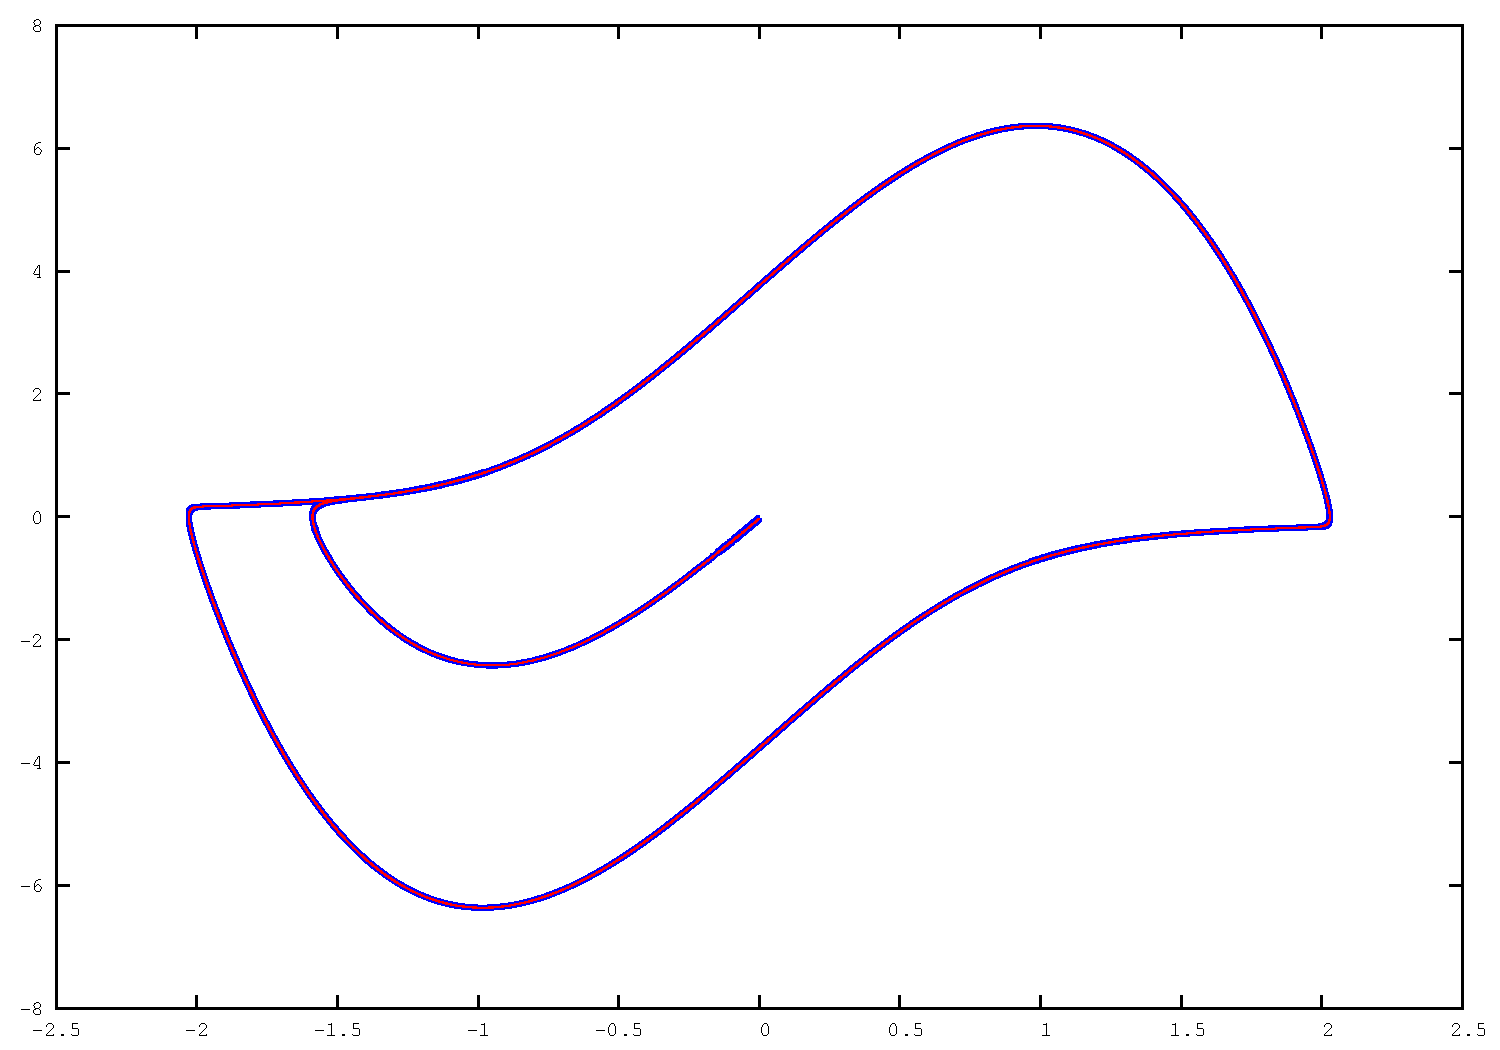
\includegraphics[width=0.75\textwidth]{vanderpol}
\caption{Traiettoria dell'oscillatore per $\mu = 4$}
\label{fig:vanderpol}
\end{figure}
Anche in questo caso si può osservare un ciclo limite nello spazio delle fasi del sistema, ovvero una traiettoria chiusa verso la quale il sistema è portato ad evolvere.

\section{Sistema di Lorenz}
\begin{figure}[H]
\centering
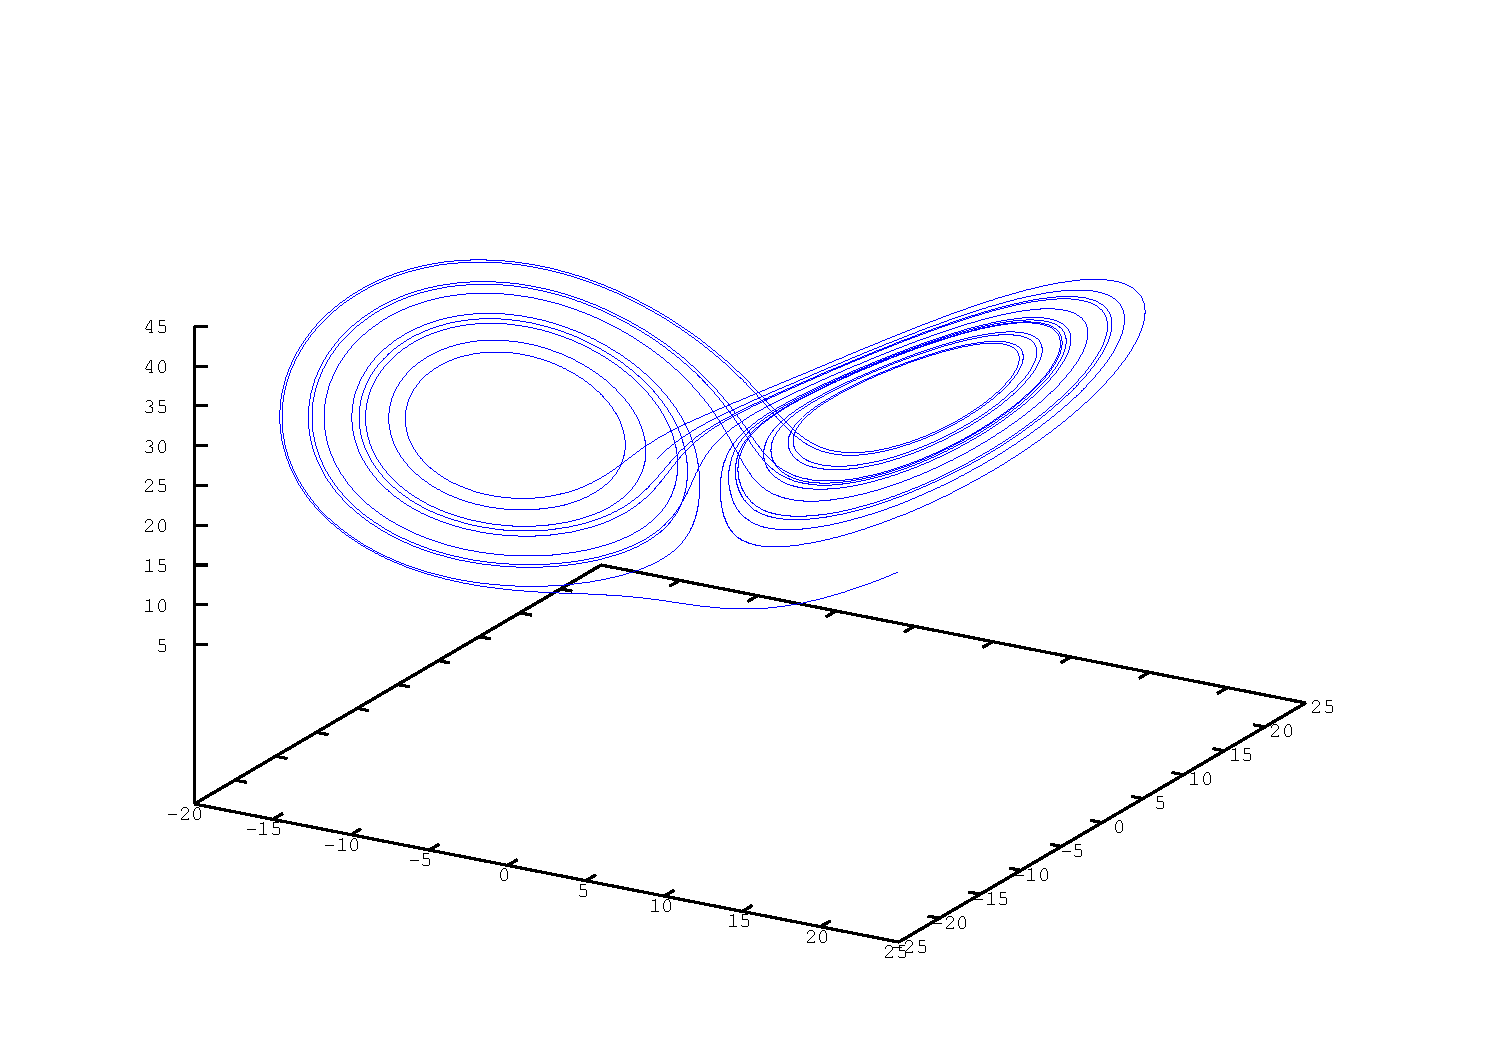
\includegraphics[width=0.33\textwidth]{lorenz0}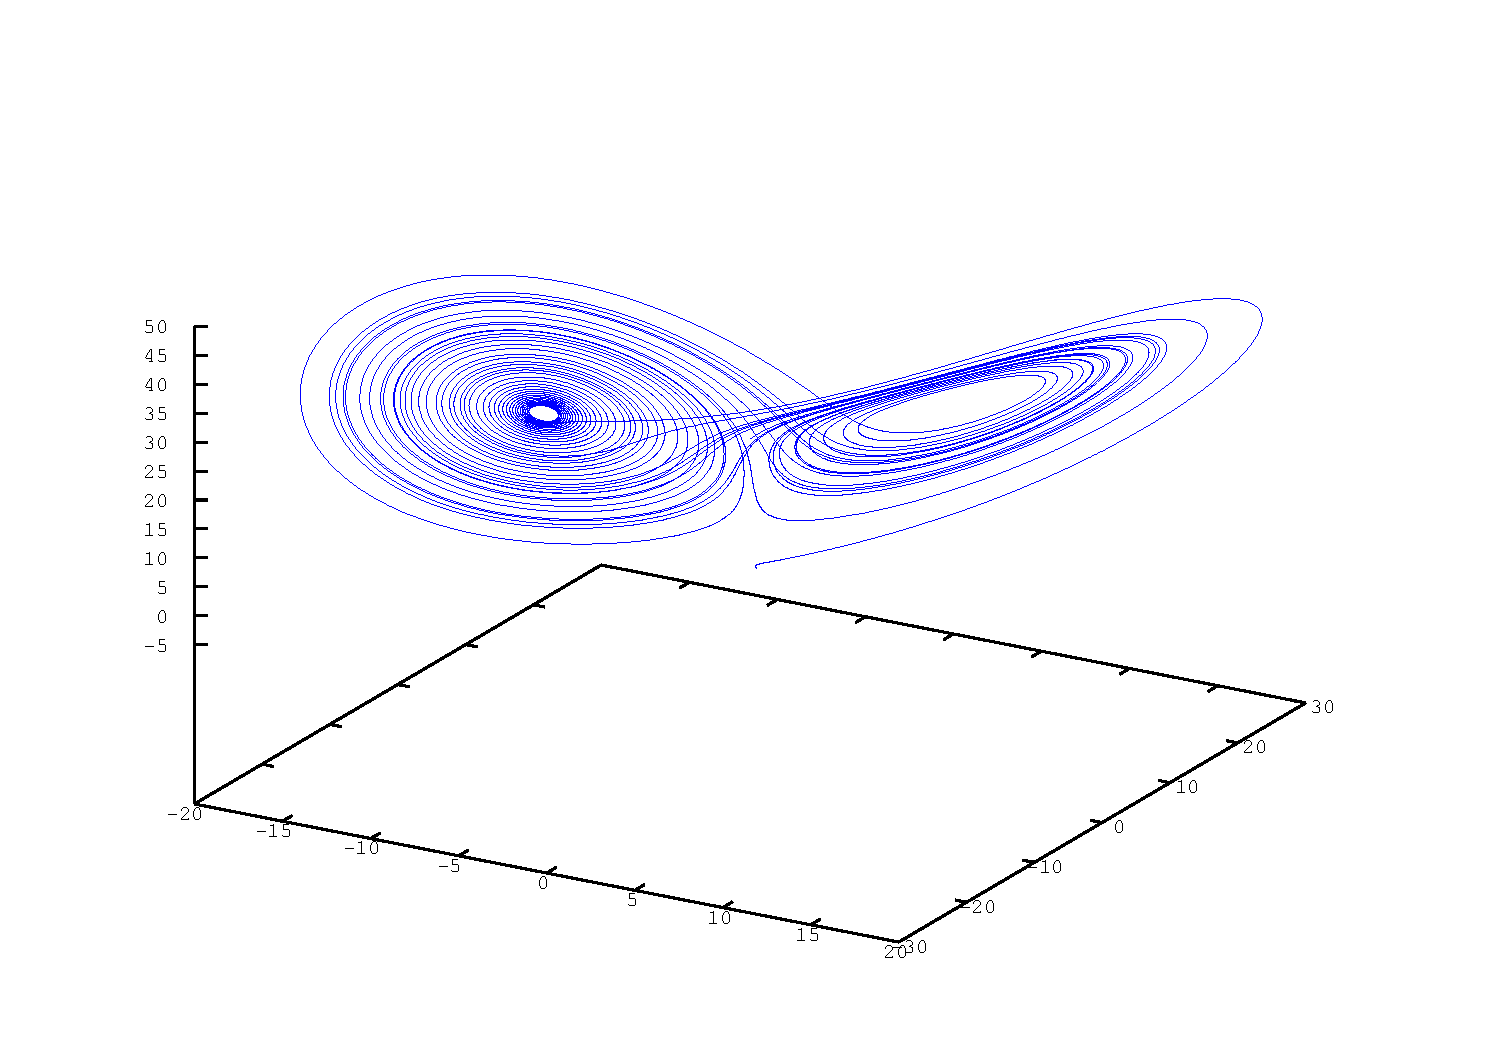
\includegraphics[width=0.33\textwidth]{lorenz1}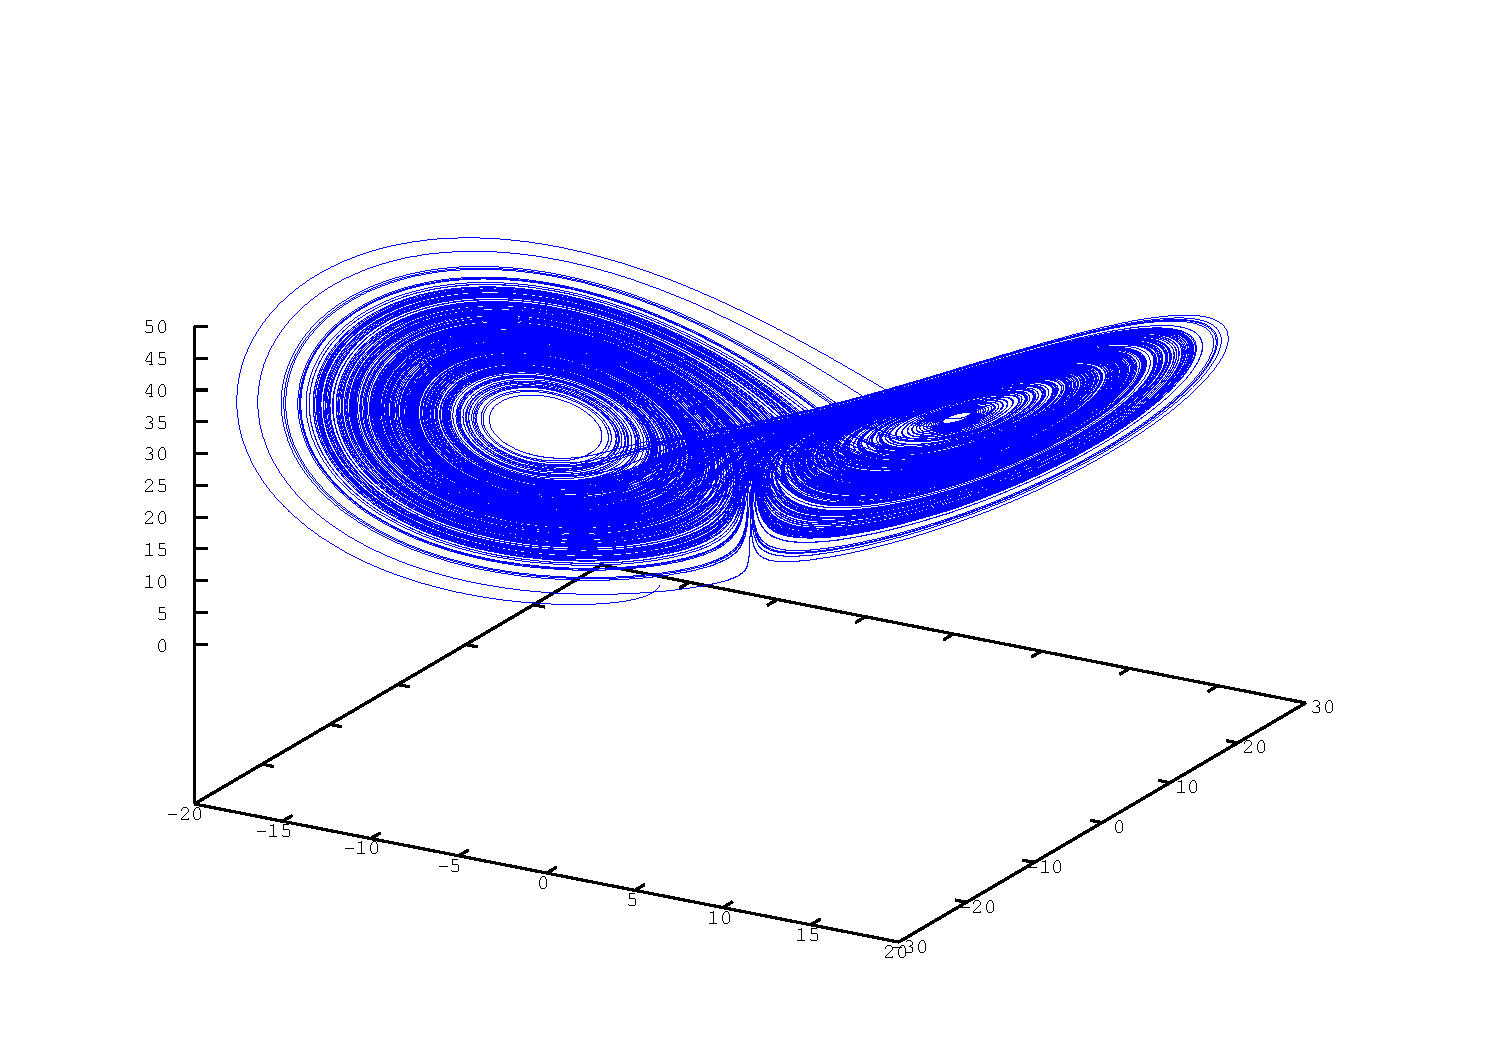
\includegraphics[width=0.33\textwidth]{lorenz2}
\caption{Sistema di Lorenz in tre dimensioni}
\label{fig:lorenz}
\end{figure}

